%%%%%%%%%%%%%%%%%%%%%%%%%%%%%%%%%%%%%%%%%%%%%%%%%%%%%%%%%%%%%%%%%%%%%%%%
%
%   SMT-COMP 2024 - 
%
%   1 hour
%
%%%%%%%%%%%%%%%%%%%%%%%%%%%%%%%%%%%%%%%%%%%%%%%%%%%%%%%%%%%%%%%%%%%%%%%%

\documentclass[table]{beamer}
\usepackage[utf8]{inputenc}
\usepackage{xcolor}
\usepackage{tikz}
\usetikzlibrary{shapes,shapes.callouts,automata,trees}
\usetikzlibrary{decorations.pathmorphing,external,fit}
\usetikzlibrary{calc}
\usetikzlibrary{backgrounds} %used for the CEGAR figure
\usepackage{amssymb}
\usepackage{clrscode}
\usepackage{pifont}
\usepackage{pdfpages}
\geometry{papersize={16cm,9cm}}
%\tikzexternalize
\usepackage{multicol}

\colorlet{MYred}{red!70!black}
\definecolor{MYgreen}{rgb}{.1,.5,0}
\definecolor{MYblue}{rgb}{0,.42,.714}
\colorlet{MYgray}{white!95!MYblue}
\colorlet{MYorange}{orange!80!black}
\definecolor{gold}{rgb}{.8,.6,0}
\colorlet{silver}{white!55!black}
\colorlet{bronze}{brown!70!black}
\def\tick{\ding{52}}
\def\cross{\ding{54}}

%%%%%%%%%%%%%%%%%%%%
%%% Beamer stuff %%%
%%%%%%%%%%%%%%%%%%%%
\usetheme{default}
\useinnertheme{rounded}
\setbeamertemplate{frametitle}[default][center]
\setbeamertemplate{footline}{\quad\hfill\footnotesize\insertframenumber\strut\kern1em\vskip2pt}
\setbeamertemplate{navigation symbols}{}
\setbeamertemplate{itemize/enumerate subbody begin}{\normalsize}
\usefonttheme[onlymath]{serif} % Nicer formulas
\setbeamercolor{block body}{bg=black!10}
\setbeamercolor{block title}{bg=black!20}

\AtBeginSection[]{
  \begin{frame}
  \vfill
  \centering
  \begin{beamercolorbox}[sep=8pt,center,shadow=true,rounded=true]{title}
    \usebeamerfont{title}\insertsectionhead\par%
  \end{beamercolorbox}
  \vfill
  \end{frame}
}

\def\emph#1{\textcolor{MYblue}{#1}}

%%% Titel, Autor und Datum des Vortrags:
\title{SMT-COMP 20243\\
19th International Satisfiability Modulo Theory Competition}
\author{Fran\c{c}ois Bobot \and \emph{Martin Bromberger} \and Martin Jon\'{a}\v{s} }
\date{July 22, 2024}

%% Institut
\institute{
CEA List, France \and
MPI für Informatik, Germany \and
Masaryk University, Czechia
}


%%%%%%%%%%%%%%%%%%%%%%%%%%%%%%%
% MACROS

% database symbol (from stackexchange)

\makeatletter
\tikzset{
    database/.style={
        path picture={
            \draw (0, 1.5*\database@segmentheight) circle [x radius=\database@radius,y radius=\database@aspectratio*\database@radius];
            \draw (-\database@radius, 0.5*\database@segmentheight) arc [start angle=180,end angle=360,x radius=\database@radius, y radius=\database@aspectratio*\database@radius];
            \draw (-\database@radius,-0.5*\database@segmentheight) arc [start angle=180,end angle=360,x radius=\database@radius, y radius=\database@aspectratio*\database@radius];
            \draw (-\database@radius,1.5*\database@segmentheight) -- ++(0,-3*\database@segmentheight) arc [start angle=180,end angle=360,x radius=\database@radius, y radius=\database@aspectratio*\database@radius] -- ++(0,3*\database@segmentheight);
        },
        minimum width=2*\database@radius + \pgflinewidth,
        minimum height=3*\database@segmentheight + 2*\database@aspectratio*\database@radius + \pgflinewidth,
    },
    database segment height/.store in=\database@segmentheight,
    database radius/.store in=\database@radius,
    database aspect ratio/.store in=\database@aspectratio,
    database segment height=0.1cm,
    database radius=0.25cm,
    database aspect ratio=0.35,
}
\makeatother


%%%%%%%%%%%%%%%%%%%%%%%%%%%%%%%

\newcommand\vitem{\vfill\item}

\begin{document}

\begin{frame}
  \titlepage
\end{frame}


\begin{frame}
  \frametitle{SMT-COMP}
  
  \begin{columns}
    \begin{column}{0.6\textwidth}
    Annual competition for \emph{SMT solvers}\\
    on (a selection of) benchmarks from \emph{SMT-LIB}
      
    \bigskip
    \bigskip    
    
    Goals:
    \begin{itemize}
      \item spur development of SMT solver implementations
      \item promote SMT solvers and their usage
      \item support the SMT-LIB project
      \begin{itemize}
        \item to promote and develop the SMT-LIB format
        \begin{itemize}
          \item model validation
          \item proof checking
        \end{itemize}
        \item to collect relevant benchmarks
      \end{itemize}
      \item engage and include new members
    \end{itemize}
    \end{column}
    \begin{column}{0.4\textwidth}
    \begin{block}{History}
      \begin{tabular}{rp{3cm}}
        \textbf{2005} & first competition \\
        \textbf{2013} & evaluation instead \\
        & of competition\\
        \textbf{2014} & since then hosted\\
        & by \emph{StarExec}\\
        \textbf{2024} & since then hosted\\
        & by \emph{BenchExec} and the \emph{SoSy-Lab} 
      \end{tabular}
    \end{block}
    \end{column}
  \end{columns}

\end{frame}

\begin{frame}
  \frametitle{SMT Solvers and SMT-LIB}
  SMT Solver
  \begin{itemize}
  \item checks formulas
    in \emph{SMT-LIB} format
    for \emph{satisfiability modulo theories}
  \end{itemize}
  \bigskip

  SMT-LIB is
  \begin{enumerate}
  \item a \emph{language} in which benchmarks are written
  \item a community effort to \emph{collect benchmarks}
  \end{enumerate}
  \medskip

  \begin{columns}
    \begin{column}{0.4\textwidth}
      \begin{block}{Non-incremental}
        438\,631 instances {\small (+4\,419)}\\ % 438631-434212=4419
        with 1 query each \\
        in 84 logics {\small (+1)}.
      \end{block}
    \end{column}
    \begin{column}{0.4\textwidth}
      \begin{block}{Incremental}
        44\,333 instances {\small (+1\,046)}\\ % 44333-43287=1046
        with 34\,069\,145 queries {\small (+32\,654)} \\ %34036491-33998935=37556
        in 39 logics. % -1 ???
      \end{block}
    \end{column}
    \begin{column}{0.08\textwidth}
    \end{column}
  \end{columns}
  \pause
    \begin{columns}
    \begin{column}{0.4\textwidth}
      \begin{block}{Selected Non-incremental}
        249\,301 instances % old 227\,940???
      \end{block}
    \end{column}
    \begin{column}{0.4\textwidth}
      \begin{block}{Selected Incremental}
        22\,826 instances % old 22\,302
      \end{block}
    \end{column}
    \begin{column}{0.08\textwidth}
    \end{column}
  \end{columns}

\end{frame}

\begin{frame}
  \frametitle{Competition Overview}

  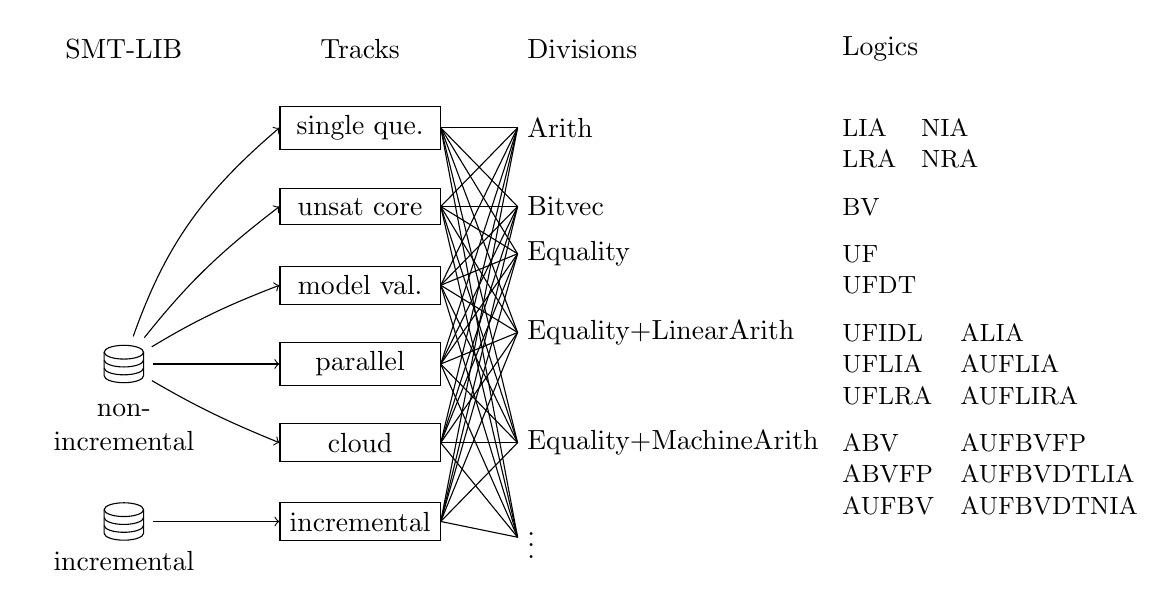
\begin{tikzpicture}
    \node at (0,6) {SMT-LIB};
    \node at (3,6) {Tracks};
    \node[anchor=west] at (5,6) {Divisions};
    \node[anchor=west] at (9,6) {Logics};

    \node[database,label=below:{\begin{tabular}{c}non-\\incremental\end{tabular}}] (nonincbench) at (0,2) {};
    \node[database,label=below:{incremental}] (incbench) at (0,0) {};

    \node[draw,text width=1.8cm,align=center](sq) at (3,5) {single que.};
    \node[draw,text width=1.8cm,align=center](uc) at (3,4) {unsat core};
    \node[draw,text width=1.8cm,align=center](mv) at (3,3) {model val.};
    \node[draw,text width=1.8cm,align=center](par) at (3,2) {parallel};
    \node[draw,text width=1.8cm,align=center](cloud) at (3,1) {cloud};
    \node[draw,text width=1.8cm,align=center](inc) at (3,0) {incremental};

    \node[anchor=west] (div1) at (5,5) {Arith};
    \node[anchor=west] at (9,5) {\small LIA};
    \node[anchor=west] at (9,4.6) {\small LRA};
    \node[anchor=west] at (10,5) {\small NIA};
    \node[anchor=west] at (10,4.6) {\small NRA};
    \node[anchor=west] (div2) at (5,4) {Bitvec};
    \node[anchor=west] at (9,4) {\small BV};
    \node[anchor=west] (div3) at (5,3.4) {Equality};
    \node[anchor=west] at (9,3.4) {\small UF};
    \node[anchor=west] at (9,3) {\small UFDT};
    \node[anchor=west] (div4) at (5,2.4) {Equality+LinearArith};
    \node[anchor=west] at (9,2.4) {\small UFIDL};
    \node[anchor=west] at (9,2) {\small UFLIA};
    \node[anchor=west] at (9,1.6) {\small UFLRA};
    \node[anchor=west] at (10.5,2.4) {\small ALIA};
    \node[anchor=west] at (10.5,2) {\small AUFLIA};
    \node[anchor=west] at (10.5,1.6) {\small AUFLIRA};
    \node[anchor=west] at (12.5,2) {$\hdots$};
    \node[anchor=west] (div5) at (5,1) {Equality+MachineArith};
    \node[anchor=west] at (9,1) {\small ABV};
    \node[anchor=west] at (9,.6) {\small ABVFP};
    \node[anchor=west] at (9,.2) {\small AUFBV};
    \node[anchor=west] at (10.5,1) {\small AUFBVFP};
    \node[anchor=west] at (10.5,.6) {\small AUFBVDTLIA};
    \node[anchor=west] at (10.5,.2) {\small AUFBVDTNIA};
    \node[anchor=west] at (12.5,1) {$\hdots$};
    \node[anchor=west] (div6)  at (5,-.2) {$\vdots$};

    \draw[->,shorten <=.3em] (nonincbench) to[bend left=15] (sq.west);
    \draw[->,shorten <=.3em] (nonincbench) to[bend left=7] (uc.west);
    \draw[->,shorten <=.3em] (nonincbench) to[bend left=5] (mv.west);
    \draw[->,shorten <=.3em] (nonincbench) to (par.west);
    \draw[->,shorten <=.3em] (nonincbench) to[bend right=4] (cloud.west);
    \draw[->,shorten <=.3em] (incbench) to (inc.west);

    \draw (sq.east) to (div1.west);
    \draw (sq.east) to (div2.west);
    \draw (sq.east) to (div3.west);
    \draw (sq.east) to (div4.west);
    \draw (sq.east) to (div5.west);
    \draw (sq.east) to (div6.west);

    \draw (uc.east) to (div1.west);
    \draw (uc.east) to (div2.west);
    \draw (uc.east) to (div3.west);
    \draw (uc.east) to (div4.west);
    \draw (uc.east) to (div5.west);
    \draw (uc.east) to (div6.west);

    \draw (mv.east) to (div1.west);
    \draw (mv.east) to (div2.west);
    \draw (mv.east) to (div3.west);
    \draw (mv.east) to (div4.west);
    \draw (mv.east) to (div5.west);
    \draw (mv.east) to (div6.west);

    \draw (cloud.east) to (div1.west);
    \draw (cloud.east) to (div2.west);
    \draw (cloud.east) to (div3.west);
    \draw (cloud.east) to (div4.west);
    \draw (cloud.east) to (div5.west);
    \draw (cloud.east) to (div6.west);

    \draw (par.east) to (div1.west);
    \draw (par.east) to (div2.west);
    \draw (par.east) to (div3.west);
    \draw (par.east) to (div4.west);
    \draw (par.east) to (div5.west);
    \draw (par.east) to (div6.west);

    \draw (inc.east) to (div1.west);
    \draw (inc.east) to (div2.west);
    \draw (inc.east) to (div3.west);
    \draw (inc.east) to (div4.west);
    \draw (inc.east) to (div5.west);
    \draw (inc.east) to (div6.west);
  \end{tikzpicture}

\end{frame}

\begin{frame}[fragile]{SMT-COMP Tracks (traditional)}
  \emph{Single Query (SQ) Track}
  \begin{itemize}
  \item Determine satisfiability of one problem
  \item Solver answers sat/unsat/unknown
  \end{itemize}
  \medskip

  \emph{Unsat Core Track}
  \begin{itemize}
  \item Find small unsatisfiable subset of input.
  \item Solver answers unsat + list of formulas.
  \end{itemize}
  \medskip

  \emph{Model Validation Track}
  \begin{itemize}
  \item Find a model for a satisfiable problem.
  \item Solver answers sat + value for each non-logical symbol.
  \end{itemize}
  \medskip

  \emph{Incremental Track}
  \begin{itemize}
  \item Solve many small problems interactively.
  \item Solver acks commands and answers sat/unsat for each check.
  \end{itemize}
\end{frame}

\begin{frame}[fragile]{SMT-COMP Tracks (experimental)}

  \emph{Model Validation}
  \begin{itemize}
    \item Division with quantifier-free floating-point logics
    \item Model validation with Dolmen (thanks to Gillaume Bury and Fran\c{c}ois
    Bobot)
  \end{itemize}
  \bigskip

  \emph{Cloud and Parallel Track} (sponsored by AWS, led by Robert Jones and Benjamin F Jones)
  \begin{itemize}
  \item Solve a large problem over the cloud (or a big computer)
  \begin{itemize}
    \item 100 machines, 1600 cores, 6400 GB of memory (cloud)
    \item 64 cores, 256 GB of memory (parallel)
  \end{itemize}
  \item Solver answers sat/unsat/unknown
  \item Thanks to Mike Whalen for managing these tracks the last two years and 
        thanks to Robert Jones and Benjamin F Jones for taking over
  \end{itemize}

\medskip
\pause
  \emph{As last year} the sat/unsat results from sound solvers in SQ were used to
  include benchmarks on the MV, UC and PE tracks.

\end{frame}

\begin{frame}[fragile]{SMT-COMP Tracks (discontinued)}

  \emph{Proof Exhibition Track}
  \begin{itemize}
  \item Solver submitted together with a checker for unsatisfiability proofs
  \item No predefined format or checker
  \item No ranking
  \item Qualitative assessment
  \item Discontinued because:
    \begin{itemize}
    \item unable to turn this into competition
    \item still processing the data of the last two years
    \item restrictions of the BenchExec cluster (no disk space to store proofs)
    \end{itemize}
  \end{itemize}
  

\end{frame}

\begin{frame}{Tracks, Solvers, Divisions, and Benchmarks}
  Teams: 20 (-5) %2023 25
  \bigskip

    \begin{tabular}{c|r@{}l|r@{}l|c}
    Track & \multicolumn{2}{c|}{Solvers} & \multicolumn{2}{c|}{Divisions}  & Benchmarks \\
    \hline
    Single Query  &  16&(-6)  & 19&(=)  & 123\,486 \\ %&(+10\,347)
    Incremental &  7&(=)   & 18&(+1)  & 22\,826   \\ %&(+525) Bitvec+Arith
    Unsat Core  &  6&(=)   & 19&(=)  & 66\,190  \\ %&(-6\,768)72\,958
    Model Validation  &  8&(-3)    &  7& (+ 8 exp.)  & 59\,625  \\ %-61\,083
%    Proof Exhibition  &  4&(=)    &  & 19 exp.  & 59\,114  \\
    \hline
    Parallel &   2&(-1)      &   &2 exp.  & 400 \\
    Cloud & 3&(+1)      &  &5 exp.  & 400 \\

  \end{tabular}
  \bigskip

  Number in parenthesis shows changes from 2023
\end{frame}

\begin{frame}
  \frametitle{Participants}

  SMT-COMP 2024 participants rely on multiple reasoning frameworks:
  \begin{itemize}
  \item CDCL(T), Saturation, MCSAT, CP
  \item automata
  \item finite domain
  \item local search
  \item besides wrappers extending the scope of existing solvers
  \end{itemize}

  \bigskip
  Six new solvers participated:
  \begin{itemize}
\item Algaroba {\footnotesize (Shah et al.)}
\item Amaya {\footnotesize (Havlena et al.)}
\item plat-smt {\footnotesize (Ewert)}
\item SMTS {\footnotesize (Kol\'{a}rik et al.)}
\item (STP-Parti-Bitwuzla {\footnotesize (Zhao et al.)})
\item Z3-Parti-Z3++ {\footnotesize (Zhao et al.)}
\end{itemize}

\end{frame}

\section{Solver Presentation}

\newcommand{\myincludepdf}[1]{
\begin{frame}
  \vspace*{-1pt}%
  \noindent\makebox[\textwidth]{%
    \includegraphics[height=\paperheight]{#1}}
\end{frame}
}

\newcommand{\myvideopdf}[2]{
\begin{frame}
  \frametitle{#1}
  \begin{center}
    video: \texttt{#2}    
  \end{center}
\end{frame}
}

\myincludepdf{amaya.pdf}

\myincludepdf{Bitwuzla.pdf}

\myincludepdf{cvc5.pdf}

\myvideopdf{OSTRICH}{Ostrich.mkv}

\myincludepdf{smtinterpol.pdf}

\myvideopdf{SMT-RAT}{SMT-RAT.mkv}

\myincludepdf{Yices2.pdf}

\myincludepdf{YicesQS.pdf}

\myincludepdf{z3-alpha.pdf}

\myincludepdf{Z3-Parti-Z3++.pdf}

\begin{frame}
    \frametitle{Other participants}
    \begin{itemize}
\item Algaroba
\vitem COLIBRI
\vitem iProver
\vitem OpenSMT
\vitem plat-smt
\vitem SMTS
\vitem STP
\vitem (STP-Parti-Bitwuzla)
\vitem Z3-Noodler
    \end{itemize}
  \end{frame}


\begin{frame}
  \frametitle{Non-Competitive Solvers}

  Submitted by organisers
  \begin{itemize}
  \item Best solvers, per division, from previous years
  \end{itemize}
  \bigskip

  Submitted by participants
  \begin{itemize}
  \item Fixed solvers (Amaya, cvc5, OSTRICH, iProver)  
  \end{itemize}
  \bigskip
  \bigskip
  (All still in the process of running)
\end{frame}

\begin{frame}{Scoring}
  Computing scores:
  \begin{itemize}
  \item \emph{Single Query/Parallel/Cloud}: number of solved \emph{instances}
  \item \emph{Incremental}: number of solved \emph{queries}
  \item \emph{Unsat Core}: number of top-level assertions \emph{removed}
  \item \emph{Model Validation}: number of solved instances with correct \emph{models}
  \end{itemize}

  \bigskip
  Error scores:
  \begin{itemize}
  \item \emph{All Tracks}: given for sat reply for unsat instance, or vice versa
  \item \emph{Unsat Core}: given if returned core is satisfiable.
  \item \emph{Model Validation}: given if given model evaluates formula to \emph{false}
  \end{itemize}
  Error scores are \textbf{draconian}.
\end{frame}

\begin{frame}{Score and Ranking}
  In each track we collect different scores:
  \begin{itemize}
  \item \emph{Sequential score} (SQ, UC, MV): all time limits apply to cpu time
  \item \emph{Parallel score} (all): all time limits apply to wallclock time
  \item \emph{SAT score} (SQ): parallel score for \emph{satisfiable} instances
  \item \emph{UNSAT score} (SQ): parallel score for \emph{unsatisfiable} instances
  \item \emph{24s} (SQ): parallel score with time limit of \emph{24s}
  \end{itemize}
  \bigskip

  Division ranking (for each score)
  \begin{itemize}
  \item For each division, one winner is declared
  \end{itemize}

  \bigskip

  Two competition-wide rankings (for each score)
  \begin{itemize}
  \item \emph{Biggest lead}: division winner with most score difference to second place
  \item \emph{Largest contribution}: improvement each solver provided to a virtual best solver
  \end{itemize}

\end{frame}

\newcommand{\seq}{\texttt{;}}
\newcommand{\paral}{\textbardbl}
\newcommand{\sat}{$\top$}
\newcommand{\unsat}{$\bot$}
\newcommand{\fast}{\texttt{24}}
\newcommand{\inc}{inc}
\newcommand{\uc}{uc}
\newcommand{\mv}{mv}
\newcommand{\cloud}{cloud}
\newcommand{\paralTrack}{parallel}

\begin{frame}
  \frametitle{Results}
  \begin{center}
    \begin{tabular}{|cl|cl|}
  \hline
  \sat & satisfiable & \unsat & unsatisfiable \\
  \seq & sequential & \paral & parallel \\
  \fast & less than 24s & \inc & incremental \\
  \uc & unsat core & \mv & model validation \\
  \hline
\end{tabular}
\end{center}
\vfill
Experimental track are added in the slides but are not present
in the certificates
\end{frame}

{
  %\newcommand{\all}{{\footnotesize (\seq,\paral,\sat,\unsat,\fast,\inc,\uc\seq,\uc\paral,\mv)}}
  \newcommand{\withtrack}[2]{\textsc{#1}{{\footnotesize (#2)}}}
  
\def\newpage{}

\newcommand{\MakeOnePage}[6]{
    \begin{frame}
    \frametitle{#1}
        
    \medskip
    \ifstrempty{#2}{}{
    \textcolor{red!30!black!90}
    {\textit{Overall Winner}}
    
    
    \textcolor{black}{\large #2}
    
     \medskip
    }

    \ifstrempty{#3}{}{
    \textcolor{red!30!black!90} {\textit{Winner of the Division#5}}
    
     \textcolor{black}{\large#3}
    
     \medskip
    }

    \ifstrempty{#4}{}{
     \textcolor{red!30!black!90}  {\textit{Winner of the Logic#6
      \ifstrempty{#3}{}{(where it did not win the corresponding division)}}}
     
     \textcolor{black}{\large #4}
    }
    \vspace{2mm}
    \end{frame}
}


\MakeOnePage{COLIBRI}{}{}{\withtrack{QF\_FP}{\unsat,\fast}, \withtrack{QF\_FPLRA}{\unsat,\fast}, \withtrack{QF\_ABVFPLRA}{\seq,\paral,\unsat,\fast}}
\newpage
\MakeOnePage{Z3++}{\withtrack{Biggest Lead}{\mv}, \withtrack{Largest Contribution}{\mv}}{\withtrack{QF\_LinearIntArith}{\seq,\paral,\sat,\mv}, \withtrack{QF\_NonLinearIntArith}{\seq,\paral,\sat,\unsat,\fast}, \withtrack{QF\_NonLinearRealArith}{\seq,\paral,\sat}}{\withtrack{QF\_IDL}{\unsat}}
\newpage
\MakeOnePage{OSTRICH}{}{}{\withtrack{QF\_S}{\seq,\paral,\unsat}}
\newpage
\MakeOnePage{SMTInterpol}{\withtrack{Biggest Lead}{\fast}}{\withtrack{QF\_Datatypes}{\fast,\uc\textsuperscript\paral}, \withtrack{QF\_Equality+LinearArith}{\seq,\paral,\sat,\inc,\mv}, \withtrack{QF\_NonLinearIntArith}{\inc}}{\withtrack{QF\_UFDT}{\uc\textsuperscript\seq}, \withtrack{QF\_UFDTLIA}{\unsat,\fast,\uc}, \withtrack{QF\_LIA}{\unsat}, \withtrack{QF\_AUFNIA}{\seq,\paral,\sat,\unsat,\fast,\uc}, \withtrack{ALIA}{\sat,\uc}, \withtrack{QF\_ANIA}{\seq,\paral,\sat,\unsat,\fast,\inc,\uc}, \withtrack{QF\_ALIA}{\uc}, \withtrack{UFLIA}{\sat}, \withtrack{QF\_UF}{\uc\textsuperscript\paral}, \withtrack{UFIDL}{\sat}, \withtrack{AUFDTLIA}{\uc}}
\newpage
\MakeOnePage{Bitwuzla}{\withtrack{Biggest Lead}{\inc}}{\withtrack{QF\_Bitvec}{\inc}, \withtrack{QF\_FPArith}{\seq,\paral,\sat,\unsat,\fast,\inc}, \withtrack{FPArith}{\seq,\paral,\sat,\unsat,\fast,\inc,\uc}, \withtrack{QF\_Equality+Bitvec}{\seq,\paral,\sat,\unsat,\fast,\inc,\mv}, \withtrack{Equality+MachineArith}{\inc}, \withtrack{Bitvec}{\sat}}{\withtrack{QF\_ABVFPLRA}{\uc}, \withtrack{ABVFP}{\sat,\fast}, \withtrack{AUFBV}{\seq,\paral,\sat,\unsat,\fast}, \withtrack{QF\_ABVFP}{\uc}, \withtrack{QF\_BVFPLRA}{\uc}, \withtrack{QF\_BVFP}{\uc}, \withtrack{ABVFPLRA}{\fast}, \withtrack{UFBVFP}{\seq,\paral,\unsat}, \withtrack{AUFBVFP}{\seq,\paral,\sat,\unsat,\fast}, \withtrack{UFBV}{\seq,\paral,\sat,\unsat,\fast}}
\newpage
\MakeOnePage{Vampire}{}{\withtrack{Equality}{\fast}}{\withtrack{UFDTNIA}{\seq,\paral,\unsat,\fast,\uc}, \withtrack{AUFLIA}{\unsat,\fast}, \withtrack{ALIA}{\seq,\paral,\unsat,\fast}, \withtrack{UFDTLIA}{\fast,\uc}, \withtrack{AUFNIRA}{\paral,\unsat,\fast}, \withtrack{UF}{\seq,\paral,\sat}, \withtrack{AUFLIRA}{\fast}}
\newpage
\MakeOnePage{Yices2}{}{\withtrack{QF\_LinearIntArith}{\fast,\inc,\uc}, \withtrack{QF\_Equality+Bitvec}{\uc}, \withtrack{QF\_Equality}{\seq,\paral,\sat,\unsat,\fast,\uc,\mv}, \withtrack{QF\_LinearRealArith}{\seq,\paral,\fast,\uc}, \withtrack{QF\_Bitvec}{\uc}, \withtrack{QF\_Equality+LinearArith}{\fast,\uc}, \withtrack{QF\_Equality+NonLinearArith}{\sat}}{\withtrack{QF\_LIRA}{\seq,\paral,\sat,\unsat,\mv}, \withtrack{QF\_UFLIA}{\unsat,\inc}, \withtrack{QF\_AUFBV}{\fast}, \withtrack{QF\_AUFBVLIA}{\inc}, \withtrack{QF\_UFLRA}{\seq,\paral,\sat,\unsat,\inc,\mv}, \withtrack{QF\_UFNRA}{\seq,\paral,\unsat,\fast,\inc,\mv}, \withtrack{QF\_UFBVLIA}{\inc}, \withtrack{QF\_RDL}{\sat,\unsat,\mv}, \withtrack{QF\_ALIA}{\unsat}, \withtrack{QF\_AUFLIA}{\seq,\paral,\sat,\unsat}}
\newpage
\MakeOnePage{YicesQS}{}{\withtrack{Arith}{\sat,\fast}}{\withtrack{LRA}{\seq,\paral,\unsat}, \withtrack{NRA}{\seq,\paral,\unsat}}
\newpage
\MakeOnePage{STP}{}{\withtrack{QF\_Bitvec}{\seq,\paral,\sat,\unsat,\fast,\mv}}{}
\newpage
\MakeOnePage{Q3B}{}{\withtrack{Bitvec}{\fast}}{}
\newpage
\MakeOnePage{cvc5}{\withtrack{Biggest Lead}{\seq,\paral,\sat,\unsat,\uc}, \withtrack{Largest Contribution}{\seq,\paral,\sat,\unsat,\fast,\inc,\uc}}{\withtrack{QF\_LinearIntArith}{\unsat}, \withtrack{QF\_Strings}{\seq,\paral,\sat,\unsat}, \withtrack{QF\_Datatypes}{\seq,\paral,\sat,\unsat,\uc\textsuperscript\seq}, \withtrack{Equality+MachineArith}{\seq,\paral,\sat,\unsat,\fast,\uc}, \withtrack{Equality}{\seq,\paral,\sat,\unsat,\inc,\uc}, \withtrack{Equality+LinearArith}{\seq,\paral,\sat,\unsat,\fast,\inc,\uc}, \withtrack{Arith}{\seq,\paral,\unsat,\inc,\uc}, \withtrack{QF\_Equality+NonLinearArith}{\seq,\paral,\unsat,\fast,\inc,\uc}, \withtrack{Bitvec}{\seq,\paral,\unsat,\inc,\uc}, \withtrack{QF\_Equality+Bitvec+Arith}{\inc}, \withtrack{Equality+NonLinearArith}{\seq,\paral,\sat,\unsat,\fast,\inc,\uc}, \withtrack{QF\_FPArith}{\uc}, \withtrack{QF\_NonLinearRealArith}{\unsat,\fast}, \withtrack{QF\_Equality}{\inc}, \withtrack{QF\_LinearRealArith}{\unsat}}{\withtrack{QF\_FP}{\sat,\mv}, \withtrack{QF\_IDL}{\uc}, \withtrack{QF\_UFNIA}{\sat}, \withtrack{LIA}{\sat,\fast}, \withtrack{UFDT}{\fast}, \withtrack{QF\_UFLRA}{\uc}, \withtrack{NIA}{\sat,\fast}, \withtrack{QF\_UFDTLIRA}{\seq,\paral,\sat,\unsat,\fast,\uc}, \withtrack{QF\_ALIA}{\inc}, \withtrack{QF\_NIRA}{\seq,\paral,\unsat}, \withtrack{QF\_UFBVDT}{\seq,\paral,\sat,\unsat,\fast}, \withtrack{QF\_AUFLIA}{\uc,\mv}, \withtrack{QF\_BVFPLRA}{\inc}, \withtrack{QF\_AX}{\mv}}
\newpage
\MakeOnePage{OpenSMT}{}{\withtrack{QF\_LinearRealArith}{\sat,\inc,\mv}, \withtrack{QF\_Equality+LinearArith}{\unsat}}{\withtrack{QF\_LIA}{\seq,\paral}, \withtrack{QF\_LRA}{\seq,\paral,\unsat,\fast}, \withtrack{QF\_UFIDL}{\seq,\paral,\sat,\mv}}
\newpage
\MakeOnePage{z3-alpha}{}{\withtrack{QF\_Strings}{\fast}}{\withtrack{QF\_S}{\sat}, \withtrack{QF\_SNIA}{\seq,\paral,\sat}}
\newpage
\MakeOnePage{iProver}{}{}{\withtrack{ANIA}{\unsat}}
\newpage


}

% \begin{frame}{Division Winners}
%   \pause
%   \emph{Single Query, sequential score}
%   \begin{itemize}
%   \item \emph{Bitwuzla}: {\small FPArith, QF\_Bitvec, QF\_Equality+Bitvec, QF\_FPArith}

%   \item \emph{cvc5}: \begin{minipage}{.8\textwidth}\raggedright \tiny Arith,
%     Bitvec, Equality, Equality+LinearArith, Equality+MachineArith,
%     Equality+NonLinearArith, QF\_Datatypes, QF\_Equality+NonLinearArith, QF\_NonLinearIntArith, QF\_NonLinearRealArith, QF\_Strings\end{minipage}

%   \item \emph{OpenSMT}: {\small QF\_LinearIntArith}

%   \item \emph{SMTInterpol}: {\small QF\_Equality+LinearArith}

%   \item \emph{Yices2}: {\small QF\_Equality, QF\_LinearRealArith}
%   \end{itemize}

%   \medskip

%   \pause
%   \emph{Unsat Core}
%   \begin{itemize}
% \item \emph{cvc5}: Arith, Bitvec, Equality+LinearArith, Equality+MachineArith,Equality+NonLinearArith,Equality(Seq), QF\_Datatypes
% \item \emph{Vampire}: Equality(Par)
% \item \emph{Bitwuzla}: QF\_EqualityBitvec, QF\_FPArith
% \item \emph{Yices2}: QF\_Bitvec, QF\_Equality+LinearArith, QF\_Equality, QF\_LinearIntArith, QF\_LinearRealArith
% \item \emph{SMTInterpol}: QF\_Equality+NonLinearArith
% \item \emph{UltimateEliminator+MathSAT}: FPArith

%   \end{itemize}

% \end{frame}

% \begin{frame}{Division Winners}
%   \emph{Incremental}
%   \begin{itemize}
% \item \emph{cvc5}: Arith, Bitvec, Equality+LinearArith,EqualityNonLinearArith,Equality
% \item \emph{UltimateEliminator+MathSAT}: Equality+MachineArith
% \item \emph{Bitwuzla}: FPArith, QF\_FPArith
% \item \emph{Yices2}: QF\_Bitvec, QF\_Equality+Bitvec, QF\_Equality, QF\_LinearIntArith
% \item \emph{SMTInterpol}: QF\_Equality+LinearArith, QF\_Equality+NonLinearArith, QF\_NonLinearIntArith
% \item \emph{OpenSMT}: QF\_LinearRealArith
%   \end{itemize}
%   \medskip

%   \pause
%   \emph{Model Validation (competitive only)}
%   \begin{itemize}
% \item \emph{Bitwuzla}: QF\_Bitvec, QF\_Equality+Bitvec,
% \item \emph{smtinterpol}: QF\_Equality+LinearArith
% \item \emph{Yices2}: QF\_Equality
% \item \emph{Z3++}: QF\_LinearIntArith
% \item \emph{OpenSMT}: QF\_LinearRealArith

% \item experimental: QF\_FPArith : Bitwuzla, cvc5

%   \end{itemize}
% \end{frame}

% \begin{frame}{Largest contribution}
%   \begin{tabular}{r|c@{}lc@{}lc@{}l}
%     &\textcolor{gold}{\textbf{1st Place}} &&
%     \textcolor{silver}{\textbf{2nd Place}} &&
%     \textcolor{bronze}{\textbf{3rd Place}}\\
%     \hline
%     \emph{Single Query}\\
%     seq & cvc5&{\tiny(Eq+MA)} & YicesQS&{\tiny(Arith)} & Bitwuzla&{\tiny(FPArith)} \\
%     par & cvc5&{\tiny(Eq+MA)} & YicesQS&{\tiny(Arith)} & Bitwuzla&{\tiny(FPArith)} \\
%     sat & cvc5&{\tiny(Eq+LA)} & YicesQS&{\tiny(Arith)} & Bitwuzla&{\tiny(FPArith)} \\
%     unsat & cvc5&{\tiny(Eq+MA)} & Z3++&{\tiny(QF\_NonLIA)} & OSTRICH&{\tiny(QF\_Strings)}\\
%     24 &  Vampire&{\tiny(Eq+NA)} & Vampire&{\tiny(Equality)} & Yices2&{\tiny(QF\_LinIA)}\\[3pt]
%     \pause
%     \emph{Incremental}\\
%     par & cvc5&{\tiny(Eq+NA)} &Yices2&{\tiny(QF\_Eq+LA)}
%     &SMTInterpol&{\tiny(QF\_Eq+NA)}\\[3pt]
%     \pause

%     \emph{Unsat Core}\\
%     seq & cvc5&{\tiny(Eq+LA)} &
%     Bitwuzla&{\tiny(QF\_Eq+Bitvec)}\\

%     par &  cvc5&{\tiny(Eq+NA)}&
%     Bitwuzla&{\tiny(QF\_Eq+Bitvec)}\\
% \\[3pt]
%     \pause
%     \emph{Model Validation}\\
%     seq &  Z3++&{\tiny(QF\_LinIA)} & Bitwuzla&{\tiny(QF\_Bitvec)}
%         & smtinterpol&{\tiny(QF\_Eq+LIA)}\\
%     par &  Z3++&{\tiny(QF\_LinIA)} & Bitwuzla&{\tiny(QF\_Bitvec)}
%         & smtinterpol&{\tiny(QF\_Eq+LIA)}\\
%   \end{tabular}
% \end{frame}


% \begin{frame}{Biggest Lead}
%   \begin{tabular}{r|c@{}lc@{}lc@{}l}
%     &\textcolor{gold}{\textbf{1st Place}} &&
%     \textcolor{silver}{\textbf{2nd Place}} &&
%     \textcolor{bronze}{\textbf{3rd Place}}\\
%     \hline
%     \emph{Single Query}\\
%     seq & cvc5&{\tiny(QF\_DT)} & Bitwuzla&{\tiny(FPArith)} & Yices2&{\tiny(QF\_LinRA)} \\
%     par & cvc5&{\tiny(QF\_DT)} & Bitwuzla&{\tiny(FPArith)} & Yices2&{\tiny(QF\_LinRA)} \\
%     sat & cvc5&{\tiny(QF\_DT)} & Bitwuzla&{\tiny(FPArith)} & Z3++&{\tiny(QF\_NonRA)} \\
%     unsat & cvc5&{\tiny(QF\_DT)} & Z3++&{\tiny(QF\_NonIA)} & Bitwuzla&{\tiny(FPArith)} \\
%     24 &  cvc5&{\tiny(Eq+MA)} & smtinterpol&{\tiny(QF\_DT)} & Vampire&{\tiny(Equality)}\\[3pt]
%     \pause
%     \emph{Incremental}\\
%     par & SMTInterpol&{\tiny(QF\_NIA)}
%     &Yices2&{\tiny(QF\_LinIA)} & cvc5&{\tiny(Eq+NonLA)} \\[3pt]
%     \pause
%     \emph{Unsat Core}\\
%     seq & cvc5&{\tiny(Eq+MA)} &    Yices2&{\tiny(QF\_Eq+LA)} &    smtinterpol&{\tiny(QF\_Eq+NA)} \\
%     par & cvc5&{\tiny(Eq+MA)} &    Yices2&{\tiny(QF\_Eq+LA)} &    smtinterpol&{\tiny(QF\_Eq+NA)} \\
%     \pause
%     \emph{Model Validation}\\
%     seq &  Z3++&{\tiny(QF\_LinIA)} & smtinterpol&{\tiny(QF\_LinA)}        & OpenSMT&{\tiny(QF\_LinRA)} \\
%     par &  Z3++&{\tiny(QF\_LinIA)} & smtinterpol&{\tiny(QF\_LinA)}        & OpenSMT&{\tiny(QF\_LinRA)} \\
%   \end{tabular}
% \end{frame}

\begin{frame}{Checking Disagreements}

  \begin{itemize}
  \item  50411 benchmarks of 249\,301 have no status

  \vitem 2 benchmarks with disagreements (QF\_SLIA)

  \vitem We manually resolved the disagreements: authors confirmed solver
  unsoundness
  \vitem We had 4 solvers with soundness issues:
    \begin{itemize}
      \item Amaya (\& Fixed)
      \item cvc5 (\& Fixed)
      \item iProver (\& Fixed)
      \item OSTRICH (\& Fixed)
    \end{itemize}
  \end{itemize}
  \end{frame}

\begin{frame}[fragile]
  \frametitle{Plans for SMT-COMP 2025?}
  \begin{itemize}
    \item General: Documentation and streamlining
    \item General: More CI support for submissions
    \item Cloud/Parallel: Integrate them into the normal process
    \item MV: Algebraic number $\implies$ non experimental
\begin{verbatim}
(root-of-with-ordering (coeffs p_0 p_1 ... p_n) i)

(root-of-with-interval  (coeffs p_0 p_1 ... p_n) min max)
(root-of-with-enclosure (coeffs p_0 p_1 ... p_n) min max)
\end{verbatim}
    Thanks for the solvers that implemented one of them!
    \item MV: partial function more discussion needed
    \item MV: array theory more discussion needed
  \end{itemize}
\end{frame}

\begin{frame}{Plans for SMT-COMP 2025?}
  \begin{itemize}
    \item Proof \textit{validation} track
      \begin{itemize}
        \item We have to analyze the data still (830gb)
        \item Ideas to turn this into a competition are welcome
      \end{itemize}

  \end{itemize}


\end{frame}

\begin{frame}{SMT-COMP organizing committee}
  Three people organize the SMT-COMP.  In 2024:
  \begin{itemize}
  \item Fran\c{c}ois Bobot
  \item Martin Bromberger
  \item Martin Jon\'{a}\v{s}
  \end{itemize}

  Martin B. has to leave early due to conflicts with his new job.\newline\newline
  Fran\c{c}ois will stay but only in an advisory role.
  \bigskip

  We need two successors for next year's competition.
  Contact us if you would like to volunteer!
\end{frame}


\begin{frame}{Acknowledgements}
  \begin{itemize}
    \item \emph{Andrea Micheli}: pysmt
    \item \emph{Guillaume Bury, FB.}: Model Validator
    \item \emph{Clark Barrett, Pascal Fontaine, Aina Niemetz, Mathias Preiner, Hans-Jörg Schurr}: SMT-LIB benchmarks
    \item \emph{Robert Jones, Benjamin F Jones, and team}: Cloud/Parallel Track
    \item \emph{Dirk Beyer and Philipp}: BenchExec and VerifierCloud support   
    \item \emph{Aaron Stump}: StarExec support
  \end{itemize}
  \bigskip

  \begin{columns}
    \begin{column}{.3\textwidth}
      \includegraphics[width=\textwidth]{starlogo}
    \end{column}
    \begin{column}{.17\textwidth}
      \includegraphics[width=\textwidth]{powered-by-aws}
    \end{column}
  \end{columns}
\end{frame}

\begin{frame}[shrink=0.95]{Benchmark contributors}
  In 2024 \emph{new benchmarks} were contributed by:

  \small
  \begin{itemize}
    \item TODO
  \end{itemize}
\end{frame}

\begin{frame}

  \begin{center}
    \Large\emph{Thanks}
  \end{center}

  \begin{center}
    to all participants
  \end{center}

  \bigskip
  \pause


  \begin{center}
    and to you for listening
  \end{center}

\end{frame}

\end{document}
